
%
\section{Tensor Core Lines} % (fold)
\label{sec:tcl_theory}
%
We define tensor core lines as the locations where eigenvector trajectories have
a locally vanishing curvature.
%
The intuition for this is similar to the intuition for the vortex core line
extractor by Sujudi and Haimes:
%
In a region where eigenvector trajectories show a swirling behavior, there must
be a center of rotation, where the swirl vanishes.
%
Similarly, an equivalent to hyperbolic trajectories~\cite{Machado2013} for
eigenvectors can be imagined.
%
Note that like vortex core lines, tensor core lines are generally not
eigenvector trajectories of the tensor field.
%
In this section, we provide a formal definition of tensor core lines and
examine their mathematical properties.
%

%
Let $\mT: \RRSet^3 \to \RRSet^{3 \times 3}$ be a \ac{3D} second-order tensor
field that may or may not be symmetric.
%
We want to find locations where the direction of a real eigenvector of $\mT$
does not change when moving along the eigenvector direction, \ie, where the
curvature of an eigenvector trajectory vanishes.
%
A vector $\vr \in \RRSet^3$ is an eigenvector of $\mT$ if $\mT\,\vr = \lambda
\vr$ for eigenvalue $\lambda \in \RRSet$ and $\vr \neq \vNull$.
%
To observe the change of eigenvector direction when moving along $\vr$,
we need to consider the derivative of $\mT$ in this direction.
%
The directional derivative of $\mT$ along $\vr$ is the linear combination
of three component-wise derivatives
%
\begin{equation*}
    \nabla_{\vr}\mT(\vx) = \nabla \mT(\vx)\,\vr = \mT_{x_1}(\vx)\, r_1
                           + \mT_{x_2}(\vx)\, r_2
                           + \mT_{x_3}(\vx)\, r_3
\end{equation*}
%
for $\vx = \T{(x_1, x_2, x_3)}$ and $\vr = \T{(r_1, r_2, r_3)}$.
%
Given $\nabla_{\vr}\mT$ we can approximate the behavior of $\mT$ along
$\vr$ as
%
\begin{equation}
\label{eq:lin_approx}
\mT(\vx + h\,\vr) = \mT(\vx) + h\, \nabla_{\vr}\mT(\vx) \,\text{,}
\end{equation}
%
with $h \in \RRSet$.
%
For our zero-curvature requirement to be fulfilled, the eigenvector direction
must not change when moving along $\vr$, \ie,
%
\begin{equation}
\label{eq:lin_cond}
    \mT(\vx + h\,\vr)\,\vr
        = \mT(\vx)\,\vr + h\, \nabla_{\vr}\mT(\vx)\,\vr
        = \mu \vr\, \text{,}
\end{equation}
%
for $\mu \in \RRSet$. This means that $\vr$ is only scaled by a factor $\mu$.
%
If we substitute $\mT(\vx)\,\vr = \lambda \vr$, we get
%
\begin{align*}
    \lambda \vr + h\, \nabla_{\vr}\mT(\vx)\,\vr &= \mu\, \vr \\
    \nabla_{\vr}\mT(\vx)\,\vr &= \frac{\mu-\lambda}{h}\, \vr\, \text{,}
\end{align*}
%
\ie, $\vr$ is also an eigenvector of $\nabla_{\vr} \mT(\vx)$.
%
With this, a tensor core line is an isolated line of positions $\vx$ where
%
\begin{equation*}
    \lambda \mT(\vx) \, \vr = \mu \nabla_{\vr}\mT(\vx)\,\vr = \vr \text{,}
\end{equation*}
%
for $\vr \neq \vNull$ and $\lambda,\, \mu \in \RRSet$.
%
In terms of the \ac{PV} operator, this equation can be expressed as
%
\begin{equation}
\label{eq:tensor_line}
    \vr \parallel \mT\,\vr \parallel \nabla_{\vr}\mT\,\vr \,\text{.}
\end{equation}
%
\begin{figure}
    \begin{captionbeside}
        {Example of seven distinct core lines in a random linear tensor field.
        \label{fig:7lines}}
        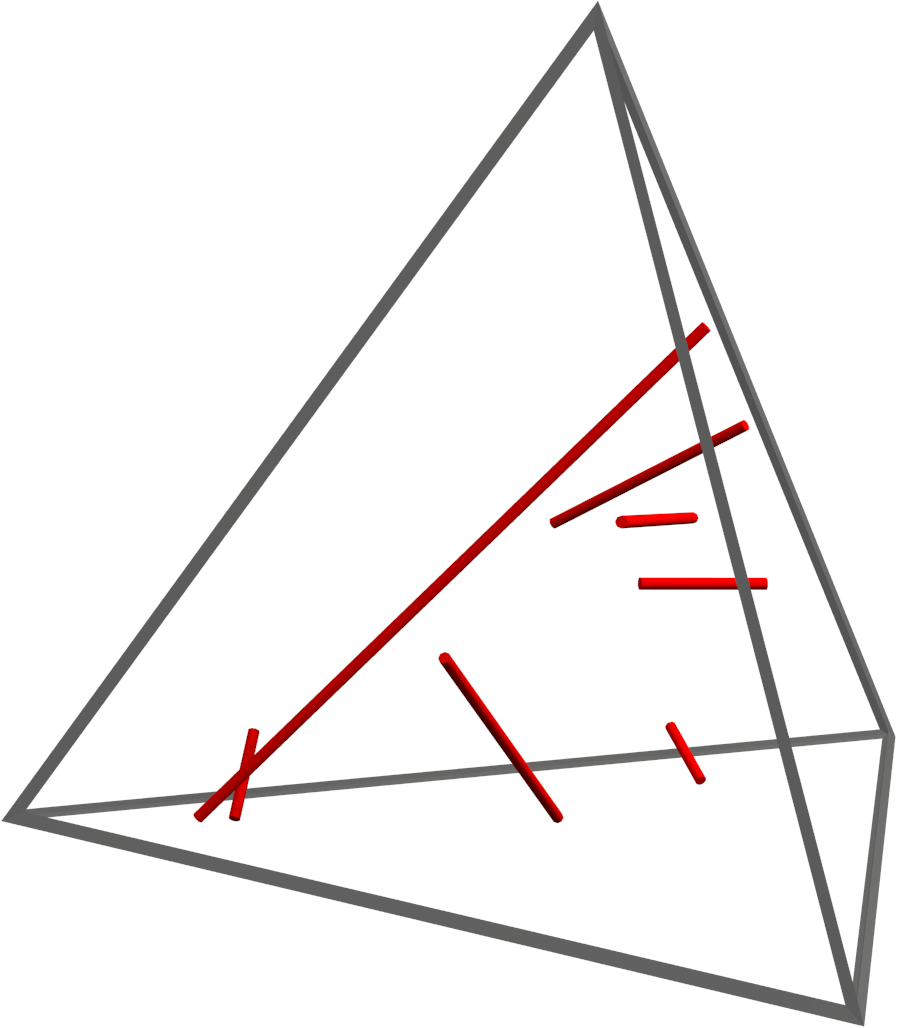
\includegraphics[width=0.5\columnwidth]{figures/7lines}
    \end{captionbeside}
\end{figure}
%

%
We now examine the mathematical properties of tensor core lines.
%

%
\begin{lemma}\label{thm:lemma1}
In a $C^1$-continuous tensor field, tensor core lines are structurally stable
line structures.
\end{lemma}
\Todo{Decide between theorem and lemma.}
%
Here, structural stability refers to the property that adding noise slightly
perturbs the structures but does not destroy them.
%
To show \cref{thm:lemma1}, we consider a local approximation of a real
eigenvector field in the neighborhood of a point as a normalized vector field.
%
Then the fact that \ac{PV} lines give line structures~\cite{Peikert1999} shows
the lemma.
%
Note that although such a consideration of an eigenvector field as a normalized
vector field is locally possible, it does not apply globally in a consistent
way, and therefore does not provide a strategy to extract tensor core lines.
\Todo{Proof done by Holger. How to handle?}
%
We also mention that in real datasets, tensor cores may build surfaces or even
parts of spatial structures.
%
This is due to shape symmetries often observed in artificial data produced by
humans.
%
Even though these structures are unstable (adding noise destroys the surfaces to
many lines), our extraction algorithm has to deal with them.
%

%
\begin{lemma}
For a linear tensor field, tensor core lines are straight lines.
\end{lemma}
%
This follows from the fact that for linear tensor fields, the linear
approximation in \eqref{eq:lin_approx} describes the whole data set
exactly: if \eqref{eq:lin_cond} holds for a small $h$, it holds for all
$h$ (i.e., on a whole straight line) as well.
%
\Cref{fig:7lines} shows an example of a random linear tensor field containing
7 isolated tensor core lines.
%